% Options for packages loaded elsewhere
% Options for packages loaded elsewhere
\PassOptionsToPackage{unicode}{hyperref}
\PassOptionsToPackage{hyphens}{url}
\PassOptionsToPackage{dvipsnames,svgnames,x11names}{xcolor}
%
\documentclass[
  letterpaper,
  DIV=11,
  numbers=noendperiod]{scrartcl}
\usepackage{xcolor}
\usepackage{amsmath,amssymb}
\setcounter{secnumdepth}{-\maxdimen} % remove section numbering
\usepackage{iftex}
\ifPDFTeX
  \usepackage[T1]{fontenc}
  \usepackage[utf8]{inputenc}
  \usepackage{textcomp} % provide euro and other symbols
\else % if luatex or xetex
  \usepackage{unicode-math} % this also loads fontspec
  \defaultfontfeatures{Scale=MatchLowercase}
  \defaultfontfeatures[\rmfamily]{Ligatures=TeX,Scale=1}
\fi
\usepackage{lmodern}
\ifPDFTeX\else
  % xetex/luatex font selection
\fi
% Use upquote if available, for straight quotes in verbatim environments
\IfFileExists{upquote.sty}{\usepackage{upquote}}{}
\IfFileExists{microtype.sty}{% use microtype if available
  \usepackage[]{microtype}
  \UseMicrotypeSet[protrusion]{basicmath} % disable protrusion for tt fonts
}{}
\makeatletter
\@ifundefined{KOMAClassName}{% if non-KOMA class
  \IfFileExists{parskip.sty}{%
    \usepackage{parskip}
  }{% else
    \setlength{\parindent}{0pt}
    \setlength{\parskip}{6pt plus 2pt minus 1pt}}
}{% if KOMA class
  \KOMAoptions{parskip=half}}
\makeatother
% Make \paragraph and \subparagraph free-standing
\makeatletter
\ifx\paragraph\undefined\else
  \let\oldparagraph\paragraph
  \renewcommand{\paragraph}{
    \@ifstar
      \xxxParagraphStar
      \xxxParagraphNoStar
  }
  \newcommand{\xxxParagraphStar}[1]{\oldparagraph*{#1}\mbox{}}
  \newcommand{\xxxParagraphNoStar}[1]{\oldparagraph{#1}\mbox{}}
\fi
\ifx\subparagraph\undefined\else
  \let\oldsubparagraph\subparagraph
  \renewcommand{\subparagraph}{
    \@ifstar
      \xxxSubParagraphStar
      \xxxSubParagraphNoStar
  }
  \newcommand{\xxxSubParagraphStar}[1]{\oldsubparagraph*{#1}\mbox{}}
  \newcommand{\xxxSubParagraphNoStar}[1]{\oldsubparagraph{#1}\mbox{}}
\fi
\makeatother


\usepackage{longtable,booktabs,array}
\newcounter{none} % for unnumbered tables
\usepackage{calc} % for calculating minipage widths
% Correct order of tables after \paragraph or \subparagraph
\usepackage{etoolbox}
\makeatletter
\patchcmd\longtable{\par}{\if@noskipsec\mbox{}\fi\par}{}{}
\makeatother
% Allow footnotes in longtable head/foot
\IfFileExists{footnotehyper.sty}{\usepackage{footnotehyper}}{\usepackage{footnote}}
\makesavenoteenv{longtable}
\usepackage{graphicx}
\makeatletter
\newsavebox\pandoc@box
\newcommand*\pandocbounded[1]{% scales image to fit in text height/width
  \sbox\pandoc@box{#1}%
  \Gscale@div\@tempa{\textheight}{\dimexpr\ht\pandoc@box+\dp\pandoc@box\relax}%
  \Gscale@div\@tempb{\linewidth}{\wd\pandoc@box}%
  \ifdim\@tempb\p@<\@tempa\p@\let\@tempa\@tempb\fi% select the smaller of both
  \ifdim\@tempa\p@<\p@\scalebox{\@tempa}{\usebox\pandoc@box}%
  \else\usebox{\pandoc@box}%
  \fi%
}
% Set default figure placement to htbp
\def\fps@figure{htbp}
\makeatother


% definitions for citeproc citations
\NewDocumentCommand\citeproctext{}{}
\NewDocumentCommand\citeproc{mm}{%
  \begingroup\def\citeproctext{#2}\cite{#1}\endgroup}
\makeatletter
 % allow citations to break across lines
 \let\@cite@ofmt\@firstofone
 % avoid brackets around text for \cite:
 \def\@biblabel#1{}
 \def\@cite#1#2{{#1\if@tempswa , #2\fi}}
\makeatother
\newlength{\cslhangindent}
\setlength{\cslhangindent}{1.5em}
\newlength{\csllabelwidth}
\setlength{\csllabelwidth}{3em}
\newenvironment{CSLReferences}[2] % #1 hanging-indent, #2 entry-spacing
 {\begin{list}{}{%
  \setlength{\itemindent}{0pt}
  \setlength{\leftmargin}{0pt}
  \setlength{\parsep}{0pt}
  % turn on hanging indent if param 1 is 1
  \ifodd #1
   \setlength{\leftmargin}{\cslhangindent}
   \setlength{\itemindent}{-1\cslhangindent}
  \fi
  % set entry spacing
  \setlength{\itemsep}{#2\baselineskip}}}
 {\end{list}}
\usepackage{calc}
\newcommand{\CSLBlock}[1]{\hfill\break\parbox[t]{\linewidth}{\strut\ignorespaces#1\strut}}
\newcommand{\CSLLeftMargin}[1]{\parbox[t]{\csllabelwidth}{\strut#1\strut}}
\newcommand{\CSLRightInline}[1]{\parbox[t]{\linewidth - \csllabelwidth}{\strut#1\strut}}
\newcommand{\CSLIndent}[1]{\hspace{\cslhangindent}#1}



\setlength{\emergencystretch}{3em} % prevent overfull lines

\providecommand{\tightlist}{%
  \setlength{\itemsep}{0pt}\setlength{\parskip}{0pt}}



 


\KOMAoption{captions}{tableheading}
\makeatletter
\@ifpackageloaded{caption}{}{\usepackage{caption}}
\AtBeginDocument{%
\ifdefined\contentsname
  \renewcommand*\contentsname{Table of contents}
\else
  \newcommand\contentsname{Table of contents}
\fi
\ifdefined\listfigurename
  \renewcommand*\listfigurename{List of Figures}
\else
  \newcommand\listfigurename{List of Figures}
\fi
\ifdefined\listtablename
  \renewcommand*\listtablename{List of Tables}
\else
  \newcommand\listtablename{List of Tables}
\fi
\ifdefined\figurename
  \renewcommand*\figurename{Figure}
\else
  \newcommand\figurename{Figure}
\fi
\ifdefined\tablename
  \renewcommand*\tablename{Table}
\else
  \newcommand\tablename{Table}
\fi
}
\@ifpackageloaded{float}{}{\usepackage{float}}
\floatstyle{ruled}
\@ifundefined{c@chapter}{\newfloat{codelisting}{h}{lop}}{\newfloat{codelisting}{h}{lop}[chapter]}
\floatname{codelisting}{Listing}
\newcommand*\listoflistings{\listof{codelisting}{List of Listings}}
\makeatother
\makeatletter
\makeatother
\makeatletter
\@ifpackageloaded{caption}{}{\usepackage{caption}}
\@ifpackageloaded{subcaption}{}{\usepackage{subcaption}}
\makeatother
\makeatletter
\@ifpackageloaded{fontawesome6}{}{\usepackage{fontawesome6}}
\makeatother
\usepackage{bookmark}
\IfFileExists{xurl.sty}{\usepackage{xurl}}{} % add URL line breaks if available
\urlstyle{same}
\hypersetup{
  pdftitle={The Psychology of Data Visualization},
  colorlinks=true,
  linkcolor={blue},
  filecolor={Maroon},
  citecolor={Blue},
  urlcolor={Blue},
  pdfcreator={LaTeX via pandoc}}


\title{The Psychology of Data Visualization}
\usepackage{etoolbox}
\makeatletter
\providecommand{\subtitle}[1]{% add subtitle to \maketitle
  \apptocmd{\@title}{\par {\large #1 \par}}{}{}
}
\makeatother
\subtitle{Fall 2026 • MWF 3:35-4:25p}
\author{}
\date{2026-07-16}
\begin{document}
\maketitle


\subsection{Spring 2025 • TTh 9:05-10:25
AM}\label{spring-2025-tth-905-1025-am}

\begin{figure}[H]

{\centering 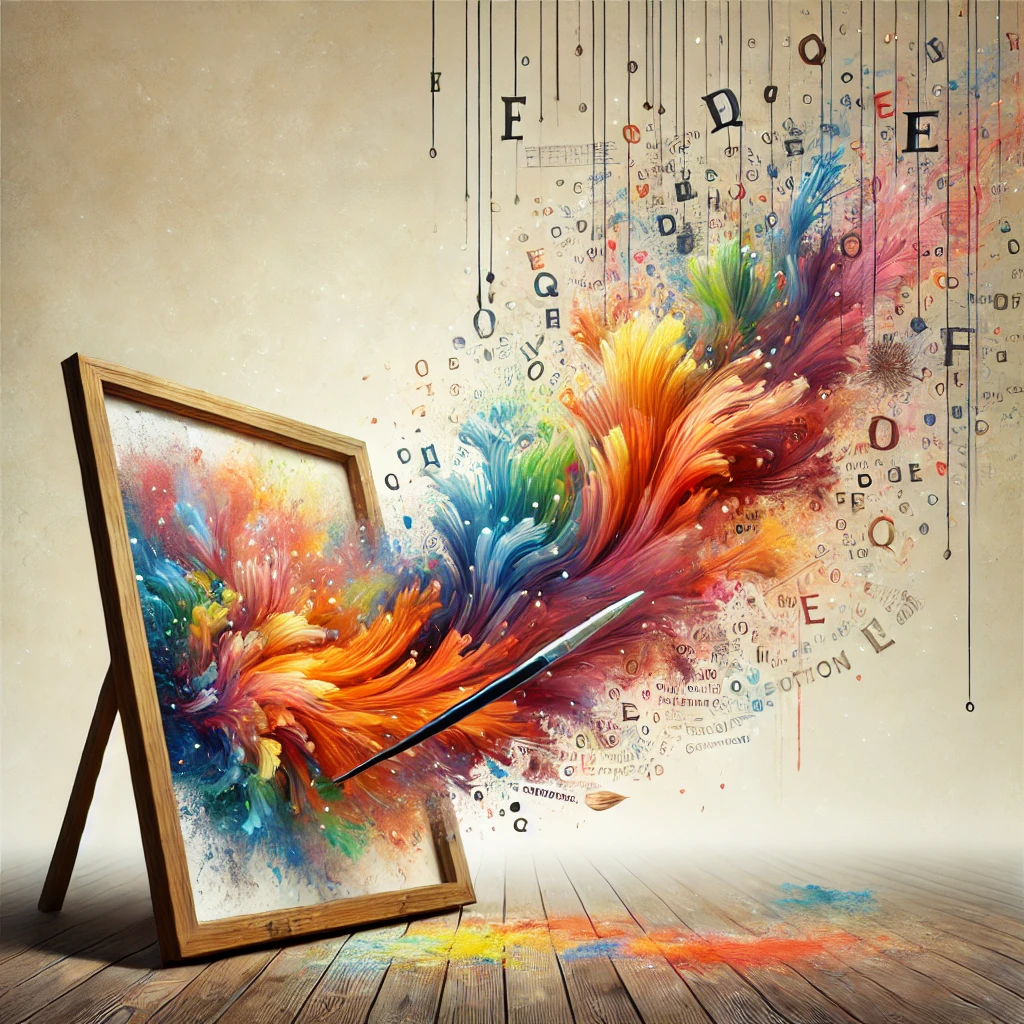
\includegraphics[width=0.5\linewidth,height=\textheight,keepaspectratio]{include/img/dall-e-2024-09-19-picture-paints.png}

}

\caption{ChatGPT/Dall-E-3 model response to `an image of ``a picture
paints a thousand words''\,' on 2024-09-19}

\end{figure}%

\subsection{Themes}\label{themes}

If a picture's worth a thousand words (Wikipedia contributors 2024a),
what exactly does it say? This course will focus on the psychology of
data visualization---how to read, critique, and generate meaningful
figures that inform but don't mislead. We'll take inspiration from
recognized classic figures and unpack what makes them exemplary. We'll
critique figures that deliberately or inadvertently mislead or confuse.
We'll learn what 150 years of vision science, the foundation of
experimental psychology, has to say about data visualization. And we'll
learn how to build our own reproducible figures using Python, R, and
JavaScript. No prior programming experience is required.

\subsection*{Instructor}\label{instructor}
\addcontentsline{toc}{subsection}{Instructor}

Rick O. Gilmore, Ph.D.~\\
Professor of Psychology\\
rog1 AT-SIGN psu PERIOD edu\\

\subsubsection{Office hours}\label{office-hours}

Monday \& Friday, 12:00p - 1:00p in 114 Moore or by appointment:
\url{https://doodle.com/mm/rickgilmore/book-a-time}

Lab web site: \url{https://gilmore-lab.github.io}

\subsection*{Teaching Assistant}\label{teaching-assistant}
\addcontentsline{toc}{subsection}{Teaching Assistant}

Kalvin Garrah\\
Graduate Student in Social Psychology\\
kmg7035 AT-SIGN psu PERIOD edu\\

\subsubsection{Office hours}\label{office-hours-1}

TBD

\subsection*{Meeting time \& location}\label{meeting-time-location}
\addcontentsline{toc}{subsection}{Meeting time \& location}

Monday, Wednesday, \& Friday, 3:35 pm - 4:25 pm\\
216
\href{https://map.psu.edu/?id=1134\#!ct/25403,26748,26749,26750,27255?m/274773?s/Osmond}{Osmond
Lab}

\subsection{Canvas site}\label{canvas-site}

Most of the course content will be found on this site.

However, we will use Canvas to track attendance, submit and grade
assignments, and provide ongoing summaries about grade point totals. The
Canvas site may be found here:

\url{https://psu.instructure.com/courses/2484925}

\subsection{Course structure}\label{course-structure}

This is a discussion-focused course. On most days we will discuss
readings assigned prior to class. On many days, we will work together or
individually on the assigned \href{index.qmd\#exercises}{exercises}, the
final project, or another assignment. Please remember to bring your
personal laptop computer. If you do not have a personal laptop, contact
Dr.~Gilmore so that we can make arrangements for you to participate
fully in the course activities.

\subsection*{Week 01}\label{week-01}
\addcontentsline{toc}{subsection}{Week 01}

\emph{Surveying the landscape}

\subsubsection*{Mon, Aug 24}\label{mon-aug-24}
\addcontentsline{toc}{subsubsection}{Mon, Aug 24}

\emph{Course introduction}

\begin{itemize}
\tightlist
\item
  \emph{Watch}:

  \begin{itemize}
  \tightlist
  \item
    PBSoffbook (2013)
  \end{itemize}
\item
  \href{slides/wk-01-2026-08-24-course-intro.qmd}{Slides}
\end{itemize}

\subsubsection*{Wed, Aug 26}\label{wed-aug-26}
\addcontentsline{toc}{subsubsection}{Wed, Aug 26}

\emph{The semiotics of data visualization}

\begin{itemize}
\tightlist
\item
  \emph{Read}:

  \begin{itemize}
  \tightlist
  \item
    Cairo (2013), Chapter 1-2,
    \href{https://psu.instructure.com/courses/2484925/files?preview=193582601}{PDF
    on Canvas}
  \end{itemize}
\item
  \emph{Assigned}: \href{exercises/ex-01-figs-in-psych-sci.qmd}{Exercise
  01} {assigned}
\item
  \href{slides/wk-01-2026-08-26-semiotics-data-viz.qmd}{Slides}
\item
  \emph{Homework}:

  \begin{itemize}
  \tightlist
  \item
    Install R and \href{https://docs.posit.co/ide/user/}{RStudio
    Desktop}

    \begin{itemize}
    \tightlist
    \item
      \href{tutorials/tutorial-install-r-rstudio.qmd}{\emph{Tutorial}}
    \end{itemize}
  \item
    (Optional) Install
    \href{https://quarto.org/docs/get-started/}{Quarto}
  \end{itemize}
\end{itemize}

\subsubsection*{Fri, Aug 28}\label{fri-aug-28}
\addcontentsline{toc}{subsubsection}{Fri, Aug 28}

\emph{Work Session: Introducing R \& RStudio}

\begin{itemize}
\tightlist
\item
  \emph{Complete}: R and RStudio Desktop installation and setup
\item
  \emph{Read}:
  \href{https://docs.posit.co/ide/user/ide/get-started/}{Get Started}
  from the RStudio User Guide.
\item
  \emph{Skim}:

  \begin{itemize}
  \tightlist
  \item
    \url{https://quarto.org/docs/get-started/hello/jupyter.html}\footnote{We
      won't use Python in this course, but the basic ideas apply to
      Python and R.}
  \item
    \url{https://education.rstudio.com/learn/beginner/}
  \end{itemize}
\item
  \href{slides/wk-01-2026-08-28-introducing-r-rstudio.qmd}{Slides}
\end{itemize}

\subsection*{Week 02}\label{week-02}
\addcontentsline{toc}{subsection}{Week 02}

\emph{Who visualizes data and why}

\subsubsection*{Mon, Aug 31}\label{mon-aug-31}
\addcontentsline{toc}{subsubsection}{Mon, Aug 31}

\emph{Visualization in government \& business}

\begin{itemize}
\tightlist
\item
  \href{slides/wk-02-2026-08-31-govt-biz.qmd}{Slides}
\end{itemize}

\subsubsection*{Wed, Sep 02}\label{wed-sep-02}
\addcontentsline{toc}{subsubsection}{Wed, Sep 02}

\emph{Visualization in art, sports, and journalism}

\begin{itemize}
\tightlist
\item
  \emph{Read}

  \begin{itemize}
  \tightlist
  \item
    Gelman and Unwin (2013) (recommended), follow citation link to
    online version or
    \href{https://psu.instructure.com/courses/2484925/files?preview=193922116}{PDF
    on Canvas}.
  \end{itemize}
\item
  {\emph{Assigned}}:
  \href{exercises/ex-02-data-viz-outside-psych.qmd}{Exercise 02}
\item
  \href{slides/slides/wk-02-2026-09-02-art-sports-journ.qmd}{Slides}
\item
  \href{404.qmd}{Results} from
  \href{exercises/ex-01-figs-in-psych-sci.qmd}{Exercise 01}
\end{itemize}

\subsubsection*{Fri, Sep 04}\label{fri-sep-04}
\addcontentsline{toc}{subsubsection}{Fri, Sep 04}

\emph{Work Session: Exercise 02 and Quarto}

\begin{itemize}
\tightlist
\item
  \faIcon{calendar} \emph{Due}
  \href{exercises/ex-01-figs-in-psych-sci.qmd}{Exercise 01} \textbar{}
  \href{https://psu.instructure.com/courses/2484925/assignments/18448425}{\faIcon{folder}
  \emph{Canvas dropbox}}
\item
  \href{404.qmd}{Slides}
\end{itemize}

\subsection*{Week 03}\label{week-03}
\addcontentsline{toc}{subsection}{Week 03}

\emph{Understanding figures}

\subsubsection*{Mon, Sep 07}\label{mon-sep-07}
\addcontentsline{toc}{subsubsection}{Mon, Sep 07}

\textbf{NO CLASS: Labor Day}

\subsubsection*{Wed, Sep 09}\label{wed-sep-09}
\addcontentsline{toc}{subsubsection}{Wed, Sep 09}

\emph{Making (sense of) data}

\begin{itemize}
\tightlist
\item
  \emph{Read}:

  \begin{itemize}
  \tightlist
  \item
    Stevens (1946) \textbar{}
    \href{https://psu.instructure.com/courses/2484925/files?preview=193582608}{PDF
    on Canvas}
  \item
    Wikipedia contributors (2024b) (Optional)
  \item
    Tourangeau et al. (2012) \textbar{}
    \href{https://psu.instructure.com/courses/2484925/files?preview=193582611}{PDF
    on Canvas}. (Optional)
  \end{itemize}
\item
  {Assigned}: \href{exercises/ex-03-making-data.qmd}{Exercise-03}
\item
  \href{404.qmd}{Slides}
\end{itemize}

\subsubsection*{Fri, Sep 11}\label{fri-sep-11}
\addcontentsline{toc}{subsubsection}{Fri, Sep 11}

\emph{Work Session: Intro to R}

\begin{itemize}
\tightlist
\item
  \href{404.qmd}{Slides}
\end{itemize}

\subsection*{Week 04}\label{week-04}
\addcontentsline{toc}{subsection}{Week 04}

\emph{The anatomy of figures}

\subsubsection*{Mon, Sep 14}\label{mon-sep-14}
\addcontentsline{toc}{subsubsection}{Mon, Sep 14}

\emph{Figure types}

\begin{itemize}
\tightlist
\item
  \emph{Explore} (pick at least two):

  \begin{itemize}
  \tightlist
  \item
    Ribecca (n.d.)
  \item
    Hammond (2024)
  \item
    Discovery (2024)
  \item
    Atlassian (n.d.)
  \end{itemize}
\item
  \emph{Watch}:

  \begin{itemize}
  \tightlist
  \item
    Channel (2024)
  \end{itemize}
\item
  \href{404.qmd}{Slides}
\end{itemize}

\subsubsection*{Wed, Sep 16}\label{wed-sep-16}
\addcontentsline{toc}{subsubsection}{Wed, Sep 16}

\emph{More figure types}

\begin{itemize}
\tightlist
\item
  \href{404.qmd}{Slides}
\end{itemize}

\subsubsection*{Fri, Sep 18}\label{fri-sep-18}
\addcontentsline{toc}{subsubsection}{Fri, Sep 18}

\emph{Work Session: Intro to ggplot}

\begin{itemize}
\tightlist
\item
  \faIcon{calendar} \emph{Due}
  \href{exercises/ex-02-data-viz-outside-psych.qmd}{Exercise 02}
  \textbar{}
  \href{https://psu.instructure.com/courses/2484925/assignments/18448429}{\faIcon{folder}
  \emph{Canvas dropbox}} \textbar{}
\item
  \href{404.qmd}{Slides}
\end{itemize}

\subsection*{Week 05}\label{week-05}
\addcontentsline{toc}{subsection}{Week 05}

\emph{Perceptual foundations}

\subsubsection*{Mon, Sep 21}\label{mon-sep-21}
\addcontentsline{toc}{subsubsection}{Mon, Sep 21}

\textbf{NO CLASS}

\subsubsection*{Wed, Sep 23}\label{wed-sep-23}
\addcontentsline{toc}{subsubsection}{Wed, Sep 23}

\emph{From stimulus to sensation}

\begin{itemize}
\tightlist
\item
  \emph{Read}:

  \begin{itemize}
  \tightlist
  \item
    Cairo (2013), Chapter 5,
    \href{https://psu.instructure.com/courses/2484925/files?preview=193582613}{PDF
    on Canvas}
  \end{itemize}
\item
  \href{404.qmd}{Slides}
\end{itemize}

\subsubsection*{Fri, Sep 25}\label{fri-sep-25}
\addcontentsline{toc}{subsubsection}{Fri, Sep 25}

\emph{Work Session: More ggplot}

\begin{itemize}
\tightlist
\item
  \faIcon{calendar} \emph{Due}
  \href{exercises/ex-03-making-data.qmd}{Exercise-03} \textbar{}
  \href{https://psu.instructure.com/courses/2484925/assignments/18448437}{\faIcon{folder}
  \emph{Canvas dropbox}} \textbar{}
\item
  \href{404.qmd}{Slides}
\end{itemize}

\subsection*{Week 06}\label{week-06}
\addcontentsline{toc}{subsection}{Week 06}

\emph{Visual perception and cognition}

\subsubsection*{Mon, Sep 28}\label{mon-sep-28}
\addcontentsline{toc}{subsubsection}{Mon, Sep 28}

\emph{From sensation to perception}

\begin{itemize}
\tightlist
\item
  \emph{Read}:

  \begin{itemize}
  \tightlist
  \item
    Cairo (2013), Chapter 6,
    \href{https://psu.instructure.com/courses/2484925/files?preview=193582613}{PDF
    on Canvas}
  \item
    Few (2004), Chapter 5,
    \href{https://psu.instructure.com/courses/2484925/files?preview=193582617}{PDF
    on Canvas}
  \end{itemize}
\item
  \emph{Optional}:

  \begin{itemize}
  \tightlist
  \item
    Cleveland and McGill (1984)\\
  \end{itemize}
\item
  \href{404.qmd}{Slides}
\end{itemize}

\subsubsection*{Wed, Sep 30}\label{wed-sep-30}
\addcontentsline{toc}{subsubsection}{Wed, Sep 30}

\emph{From cognition to understanding}

\begin{itemize}
\tightlist
\item
  \emph{Read}:

  \begin{itemize}
  \tightlist
  \item
    Franconeri et al. (2021), pp.~109-122,
    \href{https://psu.instructure.com/courses/2484925/files?preview=193922618}{PDF
    on Canvas}
  \item
    Cairo (2013), Chapter 7,
    \href{https://psu.instructure.com/courses/2484925/files?preview=193582613}{PDF
    on Canvas}
  \end{itemize}
\item
  {Assigned}: \href{exercises/final-project.qmd}{Final Project} proposal
\item
  \href{404.qmd}{Slides}
\end{itemize}

\subsubsection*{Fri, Oct 02}\label{fri-oct-02}
\addcontentsline{toc}{subsubsection}{Fri, Oct 02}

\emph{Work Session: Visualizing sports data}

\begin{itemize}
\tightlist
\item
  \faIcon{calendar} \emph{Due}
  \href{exercises/ex-04-making-figs-ggplot.qmd}{Exercise-04} \textbar{}
  \href{https://psu.instructure.com/courses/2484925/assignments/18448438}{\faIcon{folder}
  \emph{Canvas dropbox}} \textbar{}
\item
  \href{404.qmd}{Slides}
\end{itemize}

\subsection*{Week 07}\label{week-07}
\addcontentsline{toc}{subsection}{Week 07}

\subsubsection*{Mon, Oct 05}\label{mon-oct-05}
\addcontentsline{toc}{subsubsection}{Mon, Oct 05}

\emph{Exploring data}

\begin{itemize}
\tightlist
\item
  \emph{Read}:

  \begin{itemize}
  \tightlist
  \item
    Tukey (1977), Chapter 1,
    \href{https://psu.instructure.com/courses/2484925/files?preview=193922548}{PDF
    on Canvas}
  \end{itemize}
\item
  \href{404.qmd}{Slides}
\end{itemize}

\subsubsection*{Wed, Oct 07}\label{wed-oct-07}
\addcontentsline{toc}{subsubsection}{Wed, Oct 07}

\emph{Communicating uncertainty and risk}

\begin{itemize}
\tightlist
\item
  \emph{Read}:

  \begin{itemize}
  \tightlist
  \item
    Franconeri et al. (2021), pp.~139-150,
    \href{https://psu.instructure.com/courses/2484925/files?preview=193922618}{PDF
    on Canvas}
  \item
    Wilke (2019), Ch. 16\footnote{Not on Canvas yet.}
  \end{itemize}
\item
  \href{404.qmd}{Slides}
\end{itemize}

\subsubsection*{Fri, Oct 09}\label{fri-oct-09}
\addcontentsline{toc}{subsubsection}{Fri, Oct 09}

\emph{Work Session: More sports data viz}

\begin{itemize}
\tightlist
\item
  \href{404.qmd}{Slides}
\end{itemize}

\subsection*{Week 08}\label{week-08}
\addcontentsline{toc}{subsection}{Week 08}

\subsubsection*{Mon, Oct 12}\label{mon-oct-12}
\addcontentsline{toc}{subsubsection}{Mon, Oct 12}

\emph{Critiquing figures}

\begin{itemize}
\tightlist
\item
  *Read**:

  \begin{itemize}
  \tightlist
  \item
    Tufte (2001), Chapter 1,
    \href{https://psu.instructure.com/courses/2484925/files?preview=193922717}{PDF
    on Canvas}
  \item
    Tufte (2001), Chapter 2,
    \href{https://psu.instructure.com/courses/2484925/files?preview=193922717}{PDF
    on Canvas}
  \end{itemize}
\item
  \faIcon{calendar} \emph{Due} \href{exercises/final-project.qmd}{Final
  Project} proposal \textbar{}
  \href{https://psu.instructure.com/courses/2484925/assignments/18448439}{\faIcon{folder}
  \emph{Canvas dropbox}}
\item
  \href{404.qmd}{Slides}
\end{itemize}

\subsubsection*{Wed, Oct 14}\label{wed-oct-14}
\addcontentsline{toc}{subsubsection}{Wed, Oct 14}

\emph{Storytelling with data}

\begin{itemize}
\tightlist
\item
  \emph{Read}:

  \begin{itemize}
  \tightlist
  \item
    Knaflic (2015), pp.~ix-33,
    \href{https://psu.instructure.com/courses/2484925/files?preview=193922725}{PDF
    on Canvas}
  \item
    Knaflic (2015), pp.~33-69,
    \href{https://psu.instructure.com/courses/2484925/files?preview=193922725}{PDF
    on Canvas}
  \end{itemize}
\item
  \emph{Skim}: Woodside et al. (2008),
  \href{https://psu.instructure.com/courses/2484925/files?preview=193922828}{PDF
  on Canvas}
\item
  {Assigned}: \href{exercises/ex-05-tbd.qmd}{Exercise-05}
\item
  \href{404.qmd}{Slides}
\end{itemize}

\subsubsection*{Fri, Oct 16}\label{fri-oct-16}
\addcontentsline{toc}{subsubsection}{Fri, Oct 16}

\emph{Work Session: TidyTuesday or Exercise 05}

\begin{itemize}
\tightlist
\item
  \href{404.qmd}{Slides}
\end{itemize}

\subsection*{Week 09}\label{week-09}
\addcontentsline{toc}{subsection}{Week 09}

\emph{Visualizing spatial data}

\subsubsection*{Mon, Oct 19}\label{mon-oct-19}
\addcontentsline{toc}{subsubsection}{Mon, Oct 19}

\emph{Map-making}

\begin{itemize}
\tightlist
\item
  Read:

  \begin{itemize}
  \tightlist
  \item
    Wilke (2019), Chapter 15\footnote{Not on Cavnas yet.}
  \end{itemize}
\item
  \href{404.qmd}{Slides}
\end{itemize}

\subsubsection*{Wed, Oct 21}\label{wed-oct-21}
\addcontentsline{toc}{subsubsection}{Wed, Oct 21}

\begin{itemize}
\tightlist
\item
  \href{404.qmd}{Slides}
\end{itemize}

\subsubsection*{Fri, Oct 23}\label{fri-oct-23}
\addcontentsline{toc}{subsubsection}{Fri, Oct 23}

\emph{Work Session: TidyTuesday II}

\begin{itemize}
\tightlist
\item
  \href{404.qmd}{Slides}
\end{itemize}

\subsection*{Week 10}\label{week-10}
\addcontentsline{toc}{subsection}{Week 10}

\emph{Turning the table(s)}

\subsubsection*{Mon, Oct 26}\label{mon-oct-26}
\addcontentsline{toc}{subsubsection}{Mon, Oct 26}

\emph{Tables in Base R}

\begin{itemize}
\tightlist
\item
  \faIcon{calendar} \emph{Due}
  \href{exercises/ex-05-tbd.qmd}{Exercise-05}
\item
  \href{404.qmd}{Slides}
\end{itemize}

\subsubsection*{Wed, Oct 28}\label{wed-oct-28}
\addcontentsline{toc}{subsubsection}{Wed, Oct 28}

\emph{\texttt{gt} and \texttt{knitr::kable}}

\begin{itemize}
\tightlist
\item
  \href{404.qmd}{Slides}
\end{itemize}

\subsubsection*{Fri, Oct 30}\label{fri-oct-30}
\addcontentsline{toc}{subsubsection}{Fri, Oct 30}

\emph{Work Session: Tables}

\begin{itemize}
\tightlist
\item
  \href{404.qmd}{Slides}
\end{itemize}

\subsection*{Week 11}\label{week-11}
\addcontentsline{toc}{subsection}{Week 11}

\emph{Data viz in policy \& politics}

\subsubsection*{Mon, Nov 02}\label{mon-nov-02}
\addcontentsline{toc}{subsubsection}{Mon, Nov 02}

\begin{itemize}
\tightlist
\item
  \href{404.qmd}{Slides}
\end{itemize}

\subsubsection*{Wed, Nov 04}\label{wed-nov-04}
\addcontentsline{toc}{subsubsection}{Wed, Nov 04}

\begin{itemize}
\tightlist
\item
  \href{404.qmd}{Slides}
\end{itemize}

\subsubsection*{Fri, Nov 06}\label{fri-nov-06}
\addcontentsline{toc}{subsubsection}{Fri, Nov 06}

\subsection*{Week 12}\label{week-12}
\addcontentsline{toc}{subsection}{Week 12}

\subsubsection*{Mon, Nov 09}\label{mon-nov-09}
\addcontentsline{toc}{subsubsection}{Mon, Nov 09}

\subsubsection*{Wed, Nov 11}\label{wed-nov-11}
\addcontentsline{toc}{subsubsection}{Wed, Nov 11}

\subsubsection*{Fri, Nov 13}\label{fri-nov-13}
\addcontentsline{toc}{subsubsection}{Fri, Nov 13}

\emph{Work Session: More TidyTuesday}

\begin{itemize}
\tightlist
\item
  \href{404.qmd}{Slides}
\end{itemize}

\subsection*{Week 13}\label{week-13}
\addcontentsline{toc}{subsection}{Week 13}

\emph{Data viz and quantitative inference}

\subsubsection*{Mon, Nov 16}\label{mon-nov-16}
\addcontentsline{toc}{subsubsection}{Mon, Nov 16}

\emph{Synthesize before you analyze}

\begin{itemize}
\tightlist
\item
  \href{404.qmd}{Slides}
\item
  \faIcon{calendar} \emph{Due}
  \href{exercises/ex-06-tbd.qmd}{Exercise-06}
\end{itemize}

\subsubsection*{Wed, Nov 18}\label{wed-nov-18}
\addcontentsline{toc}{subsubsection}{Wed, Nov 18}

\emph{Sample size, effect size, statistical power}

\begin{itemize}
\tightlist
\item
  \href{404.qmd}{Slides}
\end{itemize}

\subsubsection*{Fri, Nov 20}\label{fri-nov-20}
\addcontentsline{toc}{subsubsection}{Fri, Nov 20}

\emph{Work Session: Final projects}

\subsection*{Thanksgiving Break}\label{thanksgiving-break}
\addcontentsline{toc}{subsection}{Thanksgiving Break}

\textbf{NO CLASS}

\subsection*{Week 14}\label{week-14}
\addcontentsline{toc}{subsection}{Week 14}

\subsubsection*{Mon, Nov 30}\label{mon-nov-30}
\addcontentsline{toc}{subsubsection}{Mon, Nov 30}

\emph{Making data dashboards and apps}

\begin{itemize}
\tightlist
\item
  Explore:

  \begin{itemize}
  \tightlist
  \item
    Kohler (2024)
  \end{itemize}
\item
  \href{404.qmd}{Slides}
\end{itemize}

\subsubsection*{Wed, Dec 02}\label{wed-dec-02}
\addcontentsline{toc}{subsubsection}{Wed, Dec 02}

\emph{Work Session: Final projects}

\subsubsection*{Fri, Dec 04}\label{fri-dec-04}
\addcontentsline{toc}{subsubsection}{Fri, Dec 04}

\emph{Work Session: Final projects}

\subsection*{Week 15}\label{week-15}
\addcontentsline{toc}{subsection}{Week 15}

\subsubsection*{Mon, Dec 07}\label{mon-dec-07}
\addcontentsline{toc}{subsubsection}{Mon, Dec 07}

\emph{Final Project Presentations}

\subsubsection*{Wed, Dec 09}\label{wed-dec-09}
\addcontentsline{toc}{subsubsection}{Wed, Dec 09}

\emph{Final Project Presentations}

\subsubsection*{Fri, Dec 11}\label{fri-dec-11}
\addcontentsline{toc}{subsubsection}{Fri, Dec 11}

\emph{Final Project Presentations}

\subsection*{Finals Week}\label{finals-week}
\addcontentsline{toc}{subsection}{Finals Week}

\subsubsection*{Wed, Dec 16}\label{wed-dec-16}
\addcontentsline{toc}{subsubsection}{Wed, Dec 16}

\begin{itemize}
\tightlist
\item
  \faIcon{calendar} \emph{Due} \href{exercises/final-project.qmd}{Final
  project} write-up \textbar{} \href{}{\faIcon{folder} \emph{Canvas
  dropbox}}
\end{itemize}

\begin{center}\rule{0.5\linewidth}{0.5pt}\end{center}

\subsection*{Elements}\label{eval-components}
\addcontentsline{toc}{subsection}{Elements}

{\def\LTcaptype{none} % do not increment counter
\begin{longtable}[]{@{}
  >{\raggedright\arraybackslash}p{(\linewidth - 4\tabcolsep) * \real{0.1667}}
  >{\raggedright\arraybackslash}p{(\linewidth - 4\tabcolsep) * \real{0.6970}}
  >{\raggedleft\arraybackslash}p{(\linewidth - 4\tabcolsep) * \real{0.1364}}@{}}
\toprule\noalign{}
\begin{minipage}[b]{\linewidth}\raggedright
Component
\end{minipage} & \begin{minipage}[b]{\linewidth}\raggedright
Description
\end{minipage} & \begin{minipage}[b]{\linewidth}\raggedleft
Points
\end{minipage} \\
\midrule\noalign{}
\endhead
\bottomrule\noalign{}
\endlastfoot
Attendance & You will receive 1 point for each class you attend up to a
maximum of 40. & 40 \\
Exercises & There will be six (6) exercises that we will work on. Each
exercise is worth 10 points. You are required to submit four (4) toward
your final grade. & 40 \\
Final project & You will complete a
\href{exercises/final-project.qmd}{final project}, either on your own,
or with a small group of 3 or fewer. Your final project is worth 40
points. & 40 \\
& \textbf{TOTAL POINTS POSSIBLE} & 120 \\
Extra Credit & If you submit more than four (4) exercise write-ups, you
may earn up to 10 extra credit points for these exercises. & \\
\end{longtable}
}

\subsection*{Grading Scheme}\label{grading-scheme}
\addcontentsline{toc}{subsection}{Grading Scheme}

{\def\LTcaptype{none} % do not increment counter
\begin{longtable}[]{@{}lcc@{}}
\toprule\noalign{}
Percent & Points & Grade \\
\midrule\noalign{}
\endhead
\bottomrule\noalign{}
\endlastfoot
94+ & 113+ & A \\
90-93 & 108-112 & A- \\
87-89 & 104-107 & B+ \\
84-86 & 100-103 & B \\
80-83 & 96-100 & B- \\
77-79 & 92-95 & C+ \\
70-76 & 84-91 & C \\
60-69 & 72-83 & D \\
\textless59 & \textless=71 & F \\
\end{longtable}
}

This page summarizes some of the key deadlines in the course.

{\def\LTcaptype{none} % do not increment counter
\begin{longtable}[]{@{}
  >{\raggedright\arraybackslash}p{(\linewidth - 2\tabcolsep) * \real{0.3333}}
  >{\raggedright\arraybackslash}p{(\linewidth - 2\tabcolsep) * \real{0.6667}}@{}}
\toprule\noalign{}
\begin{minipage}[b]{\linewidth}\raggedright
Date
\end{minipage} & \begin{minipage}[b]{\linewidth}\raggedright
What's {due}/happening
\end{minipage} \\
\midrule\noalign{}
\endhead
\bottomrule\noalign{}
\endlastfoot
\href{schedule.qmd\#fri-sep-02}{2026-09-04} &
\href{exercises/ex-01-figs-in-psych-sci.qmd}{Exercise 01} \\
\href{schedule.qmd\#fri-sep-18}{2026-09-18} &
\href{exercises/ex-02-data-viz-outside-psych.qmd}{Exercise 02} \\
\href{schedule.qmd\#fri-sep-25}{2026-09-25} &
\href{exercises/ex-03-making-data.qmd}{Exercise 03} \\
\href{schedule.qmd\#fri-oct-04}{2026-10-04} &
\href{exercises/ex-04-making-figs-ggplot.qmd}{Exercise 04} \\
\href{schedule.qmd\#mon-oct-12}{2026-10-12} &
\href{exercises/final-project.qmd}{Final project proposal} \\
\href{schedule.qmd\#mon-oct-26}{2025-10-26} &
\href{exercises/ex-05-tbd.qmd}{Exercise 05} \\
\href{schedule.qmd\#mon-nov-16}{2026-11-16} &
\href{exercises/ex-06-tbd.qmd}{Exercise 06} \\
\href{schedule.qmd\#we-dec-16}{2026-12-16} &
\href{exercises/final-project.qmd}{Final project} writeup due \\
\end{longtable}
}

Figure Figure~\ref{fig-deadlines} below shows one way to visualize these
deadlines. We'll examine it and attempt to improve it at some point in
the class.

\begin{verbatim}

Attaching package: 'dplyr'
\end{verbatim}

\begin{verbatim}
The following objects are masked from 'package:stats':

    filter, lag
\end{verbatim}

\begin{verbatim}
The following objects are masked from 'package:base':

    intersect, setdiff, setequal, union
\end{verbatim}

\begin{figure}

\centering{

\pandocbounded{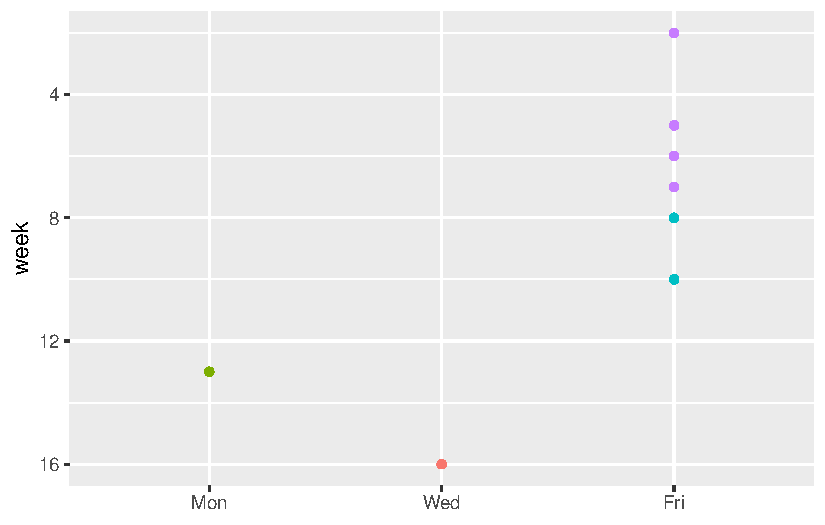
\includegraphics[keepaspectratio]{include/fig/fig-deadlines-1.pdf}}

}

\caption{\label{fig-deadlines}Visualization of assignment deadlines in
PSYCH 490.007 Fall 2026 by week of the semester, day of the week, and
month.}

\end{figure}%

\subsubsection*{Academic Integrity}\label{academic-integrity}
\addcontentsline{toc}{subsubsection}{Academic Integrity}

Students with questions about academic integrity should visit
\url{http://www.la.psu.edu/current-students/undergraduate-students/education/academic-integrity}.

Penn State defines academic integrity as the pursuit of scholarly
activity in an open, honest and responsible manner. All students should
act with personal integrity, respect others dignity, rights and
property, and help create and maintain an environment in which all can
succeed through the fruits of their efforts (Faculty Senate Policy
49-20). Sanctions for academic misconduct can include a grade of F for
the course as well as other penalties.

Unless you are told otherwise, you must complete all course work
entirely on your own, using only sources that have been permitted by
your instructor, and you may not assist other students with papers,
quizzes, exams, or other assessments. If I allow you to use ideas,
images, or word phrases created by another person (e.g., from Course
Hero or Chegg) or by generative technology, such as ChatGPT, you must
identify their source.

When you complete assignments, remember the \textbf{ABC}s to avoid
plagiarism: \textbf{A}lways place copied information within quotation
marks, include information about the quoted or paraphrased source in a
\textbf{B}ibliography, and \textbf{C}ite the source in the body (in the
text) of your paper immediately after the quoted or paraphrased
information. When in doubt, cite in the text and include the source in a
bibliography.

\textbf{Students with questions about academic integrity should ask me
or the TA before submitting work.}

Students facing allegations of academic misconduct may not drop/withdraw
from the affected course unless they are cleared of wrongdoing (see G-9:
Academic Integrity). Attempted drops will be prevented or reversed, and
students will be expected to complete course work and meet course
deadlines. Students who are found responsible for academic integrity
violations face academic outcomes, which can be severe, and put
themselves at jeopardy for other outcomes which may include
ineligibility for Dean's List, pass/fail elections, and grade
forgiveness. Students may also face consequences from their home/major
program and/or The Schreyer Honors College.

\subsubsection{Use of Artificial Intelligence
(AI)}\label{use-of-artificial-intelligence-ai}

You may use AI tools to assist with your work, but you must properly
cite any sources used. This includes AI-generated content, such as text,
images, data, or code.

Always ensure that your work reflects your own understanding and that
you are not relying solely on AI tools to complete assignments.

If you do make use of AI, please cite the AI tool used and provide a
brief description of how it was used in your work. Please also save a
transcript of your interaction with the AI tool and submit that as an
appendix to your assignment.

See \url{https://integrity.psu.edu/ai} for more details, and when in
doubt, please ask the instructor or TA.

\subsubsection*{Absences or late
assignments}\label{late-missed-assignments}
\addcontentsline{toc}{subsubsection}{Absences or late assignments}

\paragraph{Absence from class}\label{absence-from-class}

Your absence from class may be excused under unusual circumstances such
as (a) an interview for graduate school or a job, (b) illness, (c)
religious observance, (d) the death of a family member, or (e) any other
event recognized by the university as a valid excuse for absence from
class.

If you must miss class, you must contact the instructor and the TA
\textbf{in advance}.

Up to three (3) excused absences will be permitted.

\paragraph*{Late exercises}\label{late-exercises}
\addcontentsline{toc}{paragraph}{Late exercises}

Exercises submitted after the published deadlines will not be eligible
for full credit unless the instructor has given specific permission.

\paragraph*{Late final projects}\label{late-final-projects}
\addcontentsline{toc}{paragraph}{Late final projects}

Final projects submitted after the published deadline will not be
eligible for full credit unless the instructor has given specific
permission.

\paragraph*{Accommodation for persons with
disabilities}\label{disability-accommodations}
\addcontentsline{toc}{paragraph}{Accommodation for persons with
disabilities}

Penn State welcomes students with disabilities into the University's
educational programs. Please refer to the information provided by
Student Disability Resources (SDR) at
\url{http://equity.psu.edu/student-disability-resources/} for
information about the procedures required to obtain reasonable
accommodations in this course. Students should discussSDR-approved
accommodations with their instructor as early in the semester as
possible, even if they have taken another course with the instructor.
Please note: students are not required to provide their instructor with
information about the nature of their condition.

Penn State students are also welcome to contact other units for
assistance with personal concerns that interfere with academic progress,
including: Counseling and Psychological Services (CAPS;
\url{http://studentaffairs.psu.edu/counseling/}), the Office of Student
Affairs (\url{http://studentaffairs.psu.edu/}), Career Services
(\url{http://studentaffairs.psu.edu/career/}), the Center for Women
Students (\url{http://studentaffairs.psu.edu/womenscenter/}), the LGBTQA
Student Resource Center (\url{http://studentaffairs.psu.edu/lgbtqa/}),
the Office of Sexual Misconduct Prevention and Response
(\url{http://titleix.psu.edu/}), Penn State Educational Equity
(\url{http://equity.psu.edu/}), the Multicultural Resource Center
(\url{http://equity.psu.edu/mrc}), and University Health Services
(\url{http://studentaffairs.psu.edu/health/}).

\subsubsection*{Nondiscrimination
Statement}\label{non-discrimination-statement}
\addcontentsline{toc}{subsubsection}{Nondiscrimination Statement}

The Pennsylvania State University is committed to equal access to
programs, facilities, admission and employment for all persons. It is
the policy of the University to maintain an environment free of
harassment and free of discrimination against any person because of age,
race, color, ancestry, national origin, religion, creed, service in the
uniformed services (as defined in state and federal law), veteran
status, sex, sexual orientation, marital or family status, pregnancy,
pregnancy-related conditions, physical or mental disability, gender,
perceived gender, gender identity, genetic information or political
ideas.\\
Discriminatory conduct and harassment, as well as sexual misconduct and
relationship violence, violates the dignity of individuals, impedes the
realization of the University's educational mission, and will not be
tolerated.

Direct all inquiries regarding the nondiscrimination policy to:

Suzanne C. Adair Associate Vice President for Equal Opportunity and
Access Office of Equal Opportunity and Access The Pennsylvania State
University 328 Boucke Building University Park, PA 16802-5901 Email:
sca917@psu.edu Tel (814) 863-0471

\subsubsection*{Diversity Statement}\label{diversity-statement}
\addcontentsline{toc}{subsubsection}{Diversity Statement}

This classroom is a place where you will be treated with respect. All
members of this class are expected to contribute to a respectful,
welcoming and inclusive environment for every other member of the
class.\\
Penn State is committed to creating an educational environment which is
free from intolerance directed toward individuals or groups and strives
to create and maintain an environment that fosters respect for others as
stated in Policy AD29 Statement on Intolerance.

\subsubsection*{Mandated Reporting Statement}\label{mandated}
\addcontentsline{toc}{subsubsection}{Mandated Reporting Statement}

Penn State's policies require me, as a faculty member, to share
information about incidents of sex-based discrimination and harassment
(discrimination, harassment, sexual harassment, sexual misconduct,
dating violence, domestic violence, stalking, and retaliation) with Penn
State's Title IX coordinator or deputy coordinators, regardless of
whether the incidents are stated to me in person or shared by students
as part of their coursework. For more information regarding the
University's policies and procedures for responding to reports of sexual
or gender-based harassment or misconduct, please visit
\url{http://titleix.psu.edu}.

Additionally, I am required to make a report on any reasonable suspicion
of child abuse in accordance with the Pennsylvania Child Protective
Services Law.

\subsubsection*{Zoom}\label{zoom}
\addcontentsline{toc}{subsubsection}{Zoom}

At some point in the semester, I may decide to use Zoom to allow
students who are unable to attend class in person to participate.

While you are on Zoom, keep in mind that this is a classroom environment
and others should be treated with respect. Please keep your microphone
muted unless you want to ask a question or interact with someone. If
your microphone is not muted, the entire class will be able to hear what
is going on in your environment. As an instructor, I personally like to
see people's faces. As a participant, I am more involved when I have my
camera on. I realize, however, that there are many reasons why you might
not want to turn on your camera such as poor internet connection,
joining via phone, or other privacy concerns. It is your choice as to
whether you would like to have the camera on or not.

\subsection{Values}\label{values}

\subsubsection*{Penn State Principles}\label{psu-principles}
\addcontentsline{toc}{subsubsection}{Penn State Principles}

The Pennsylvania State University is a community dedicated to personal
and academic excellence. The Penn State Principles were developed to
embody the values that we hope our students, faculty, staff,
administration, and alumni possess. At the same time, the University is
strongly committed to freedom of expression. Consequently, these
Principles do not constitute University policy and are not intended to
interfere in any way with an individual's academic or personal freedoms.
We hope, however, that individuals will voluntarily endorse these common
principles, thereby contributing to the traditions and scholarly
heritage left by those who preceded them, and will thus leave Penn State
a better place for those who follow.

\textbf{I will respect the dignity of all individuals within the Penn
State community}. The University is committed to creating and
maintaining an educational environment that respects the right of all
individuals to participate fully in the community. Actions motivated by
hate, prejudice, or intolerance violate this principle. I will not
engage in any behaviors that compromise or demean the dignity of
individuals or groups, including intimidation, stalking, harassment,
discrimination, taunting, ridiculing, insulting, or acts of violence. I
will demonstrate respect for others by striving to learn from
differences between people, ideas, and opinions and by avoiding
behaviors that inhibit the ability of other community members to feel
safe or welcome as they pursue their academic goals.

\textbf{I will practice academic integrity}. Academic integrity is a
basic guiding principle for all academic activity at Penn State
University, allowing the pursuit of scholarly activity in an open,
honest, and responsible manner. In accordance with the University Code
of Conduct, I will practice integrity in regard to all academic
assignments. I will not engage in or tolerate acts of falsification,
misrepresentation or deception because such acts of dishonesty violate
the fundamental ethical principles of the University community and
compromise the worth of work completed by others.

\textbf{I will demonstrate social and personal responsibility}. The
University is a community that promotes learning; any behaviors that are
inconsistent with that goal are unacceptable. Irresponsible behaviors,
including alcohol or drug abuse and the use of violence against people
or property, undermine the educational climate by threatening the
physical and mental health of members of the community. I will exercise
personal responsibility for my actions and I will make sure that my
actions do not interfere with the academic and social environment of the
University. I will maintain a high standard of behavior by adhering to
the Code of Conduct and respecting the rights of others.

\textbf{I will be responsible for my own academic progress and agree to
comply with all University policies}. The University allows students to
identify and achieve their academic goals by providing the information
needed to plan the chosen program of study and the necessary educational
opportunities, but students assume final responsibility for course
scheduling, program planning, and the successful completion of
graduation requirements. I will be responsible for seeking the academic
and career information needed to meet my educational goals by becoming
knowledgeable about the relevant policies, procedures, and rules of the
University and academic program, by consulting and meeting with my
adviser, and by successfully completing all of the requirements for
graduation.

\subsubsection*{Penn State Values}\label{psu-values}
\addcontentsline{toc}{subsubsection}{Penn State Values}

\href{http://universityethics.psu.edu/examples-action\#integrityexamples}{\textbf{Integrity}}:
We act with integrity and honesty in accordance with the highest
academic, professional, and ethical standards.

\href{http://universityethics.psu.edu/examples-action\#respectexamples}{\textbf{Respect}}:
We respect and honor the dignity of each person, embrace civil
discourse, and foster a diverse and inclusive community.

\href{http://universityethics.psu.edu/examples-action\#responsibilityexamples}{\textbf{Responsibility}}:
We act responsibly, and we are accountable for our decisions, actions,
and their consequences.

\href{http://universityethics.psu.edu/examples-action\#discoveryexamples}{\textbf{Discovery}}:
We seek and create new knowledge and understanding, and foster
creativity and innovation, for the benefit of our communities, society,
and the environment.

\href{http://universityethics.psu.edu/examples-action\#excellenceexamples}{\textbf{Excellence}}:
We strive for excellence in all our endeavors as individuals, an
institution, and a leader in higher education.

\href{http://universityethics.psu.edu/examples-action\#communityexamples}{\textbf{Community}}:
We work together for the betterment of our University, the communities
we serve, and the world.

\subsection*{References}\label{references}
\addcontentsline{toc}{subsection}{References}

\protect\phantomsection\label{refs}
\begin{CSLReferences}{1}{1}
\bibitem[\citeproctext]{ref-AtlassianUnknown-ob}
Atlassian. n.d. {``Essential Chart Types for Data Visualization.''}
Accessed January 24, 2025.
\url{https://www.atlassian.com/data/charts/essential-chart-types-for-data-visualization}.

\bibitem[\citeproctext]{ref-Cairo2013-hm}
Cairo, Alberto. 2013. \emph{The Functional Art: An Introduction to
Information Graphics and Visualization}. New Riders Publishing.

\bibitem[\citeproctext]{ref-Channel2024-so}
Channel, Mconsultingprep Official. 2024. \emph{Every {CHART} Types
Explained in 12 Minutes}. You{T}ube.
\url{https://www.youtube.com/watch?v=cuMwWvtNmJ0}.

\bibitem[\citeproctext]{ref-Cleveland1984-py}
Cleveland, William S, and Robert McGill. 1984. {``Graphical Perception:
Theory, Experimentation, and Application to the Development of Graphical
Methods.''} \emph{Journal of the American Statistical Association} 79
(September): 531--54.
\url{https://doi.org/10.1080/01621459.1984.10478080}.

\bibitem[\citeproctext]{ref-Discovery2024-la}
Discovery, Jmp Statistical. 2024. {``Types of Graphs.''} January 4.
\url{https://www.jmp.com/en_us/statistics-knowledge-portal/exploratory-data-analysis/types-of-graphs.html}.

\bibitem[\citeproctext]{ref-Stephen-Few2004-jv}
Few, Stephen. 2004. \emph{Show Me the Numbers: Designing Tables and
Graphs to Enlighten}. Analytics Press.

\bibitem[\citeproctext]{ref-Franconeri2021-uv}
Franconeri, Steven L, Lace M Padilla, Priti Shah, Jeffrey M Zacks, and
Jessica Hullman. 2021. {``The Science of Visual Data Communication: What
Works.''} \emph{Psychological Science in the Public Interest: A Journal
of the American Psychological Society} 22 (3): 110--61.
\url{https://doi.org/10.1177/15291006211051956}.

\bibitem[\citeproctext]{ref-Gelman2013-he}
Gelman, Andrew, and Antony Unwin. 2013. {``Infovis and Statistical
Graphics: Different Goals, Different Looks.''} \emph{Journal of
Computational and Graphical Statistics: A Joint Publication of American
Statistical Association, Institute of Mathematical Statistics, Interface
Foundation of North America} 22 (January): 2--28.
\url{https://doi.org/10.1080/10618600.2012.761137}.

\bibitem[\citeproctext]{ref-Hammond2024-ow}
Hammond, Tony. 2024. {``20 Types of Charts and Graphs for Data
Visualization.''} November 26.
\url{https://www.thoughtspot.com/data-trends/data-visualization/types-of-charts-graphs}.

\bibitem[\citeproctext]{ref-Knaflic2015-wq}
Knaflic, Cole Nussbaumer. 2015. \emph{Storytelling with Data}. John
Wiliey \& Sons.

\bibitem[\citeproctext]{ref-Kohler2024-ig}
Kohler, Tanner. 2024. {``Psychology for {UX}: Study Guide.''} January
10. \url{https://www.nngroup.com/articles/psychology-study-guide/}.

\bibitem[\citeproctext]{ref-PBSoffbook2013-zh}
PBSoffbook. 2013. \emph{The Art of Data Visualization \textbar{} Off
Book \textbar{} {PBS} Digital Studios}. You{T}ube.
\url{https://www.youtube.com/watch?v=AdSZJzb-aX8&t=3s}.

\bibitem[\citeproctext]{ref-RibeccaUnknown-tz}
Ribecca, Severino. n.d. {``The Data Visualisation Catalogue.''} Accessed
January 24, 2025. \url{https://datavizcatalogue.com/index.html}.

\bibitem[\citeproctext]{ref-Stevens1946-sh}
Stevens, S S. 1946. {``On the Theory of Scales of Measurement.''}
\emph{Science (New York, N.Y.)} 103 (June): 677--80.
\url{https://doi.org/10.1126/science.103.2684.677}.

\bibitem[\citeproctext]{ref-Tourangeau2012-fr}
Tourangeau, Roger, Lance J Rips, and Kenneth Rasinski. 2012. \emph{The
{P}sychology of {S}urvey {R}esponse}. Cambridge University Press.
\url{https://doi.org/10.1017/cbo9780511819322}.

\bibitem[\citeproctext]{ref-Tufte2001-cb}
Tufte, Edward R. 2001. \emph{The {V}isual {D}isplay of {Q}uantitative
{I}nformation}. Graphics Pr.

\bibitem[\citeproctext]{ref-Tukey1977-ro}
Tukey, John W. 1977. \emph{Exploratory Data Analysis}. Addison-Wesley
Series in Behavioral Science. Quantitative Methods. Pearson.
\url{https://www.amazon.com/Exploratory-Data-Analysis-John-Tukey/dp/0201076160}.

\bibitem[\citeproctext]{ref-Wikipedia-contributors2024-du}
Wikipedia contributors. 2024a. \emph{A Picture Is Worth a Thousand
Words}.
\href{https://en.wikipedia.org/wiki/A_picture_is_worth_a_thousand_words}{Https://en.wikipedia.org/wiki/A\_picture\_is\_worth\_a\_thousand\_words};
Wikimedia Foundation, Inc.

\bibitem[\citeproctext]{ref-Wikipedia-contributors2024-xu}
Wikipedia contributors. 2024b. {``Statistical Data Type.''} Wikimedia
Foundation, Inc., November 23.
\url{https://en.wikipedia.org/wiki/Statistical_data_type}.

\bibitem[\citeproctext]{ref-Wilke2019-mx}
Wilke, Claus O. 2019. \emph{Fundamentals of Data Visualization: A Primer
on Making Informative and Compelling Figures}. O'Reilly Media.
\url{https://www.amazon.com/Fundamentals-Data-Visualization-Informative-Compelling/dp/1492031089}.

\bibitem[\citeproctext]{ref-Woodside2008-yv}
Woodside, Arch G, Suresh Sood, and Kenneth E Miller. 2008. {``When
Consumers and Brands Talk: Storytelling Theory and Research in
Psychology and Marketing.''} \emph{Psychology \& Marketing} 25
(February): 97--145. \url{https://doi.org/10.1002/mar.20203}.

\end{CSLReferences}




\end{document}
